\subsection{Modelo MM1 en AnyLogic}

\begin{figure}[H]
  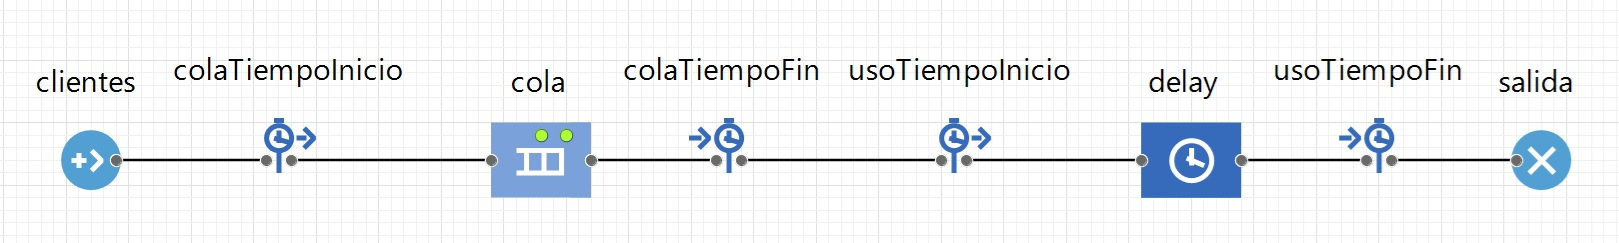
\includegraphics[width=\linewidth]{images/anylogic-colas-modelo}
  \caption{Bloques del modelo MM1 en Anylogic.}
\end{figure}

Para analizar el rendimiento del modelo, variamos la tasa de arribos ($T_a$) en base a la tasa de servicio ($T_s$) y
la capacidad de la cola ($cap$).

Realizaremos 10 simulaciones de 1000 clientes cada una y promediamos los siguientes estadísticos:
\begin{itemize}
    \item Demora promedio esperada en cola ($d(n)$)
    \item Cantidad de clientes en cola en promedio ($q(n)$)
    \item Ocupación del servidor ($u(n)*100\%$)
    \item Promedio de clientes en el sistema ($q(n)+u(n)$)
    \item Probabilidad de denegación del servicio. ($p(den)$)
    \item Probabilidad de encontrar n clientes en cola. ($p(Q(t)=n)\times100\%$)
\end{itemize}

Los primeros 5 fueron tabulados y el último fue graficado.

\subsubsection{$T_a = 25\% * T_s$}

\begin{tabular}{||c|c|c|c|c|c||}
    \hline \hline
    $cap$ & $d(n)$ & $q(n)$ & $u(n)\times100\%$ & $q(n)+u(n)$ & $p(den)$ \\
    \hline \hline
    0 & N/A & N/A & $19,8$ & $1,98$ & $20,16$ \\
    \hline
    2 & $0,5771$ & $0,0718$ & $24,8$ & $2,5728$ & $1,21$ \\
    \hline
    5 &  &  &  &  &  \\
    \hline
    10 &  &  &  &  &  \\
    \hline
    50 &  &  &  &  &  \\
    \hline
    $\infty$ &  &  &  &  & N/A \\
    \hline \hline
\end{tabular}
